\documentclass[tikz,border=5pt]{standalone}
\usepackage{luatexja-fontspec}
\setmainjfont{Hiragino Mincho ProN}
\setsansjfont{Hiragino Sans}
\usepackage{amsmath}
\usetikzlibrary{arrows.meta}

\begin{document}
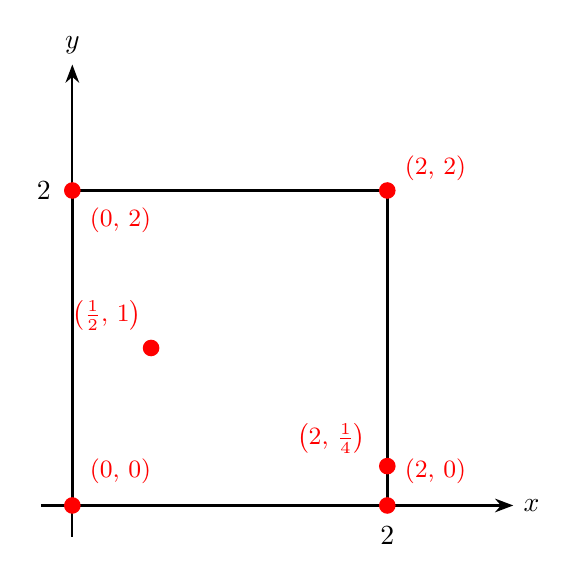
\begin{tikzpicture}[
  every node/.style={font=\normalsize},
  plabel/.style={font=\small, text=red},
]

% Scale: 1 unit = 2cm
\def\s{2.0}

% Axes
\draw[-{Stealth}, thick] (-0.4, 0) -- (2.8*\s, 0) node[right] {$x$};
\draw[-{Stealth}, thick] (0, -0.4) -- (0, 2.8*\s) node[above] {$y$};

% Axis labels
\node[below] at (2*\s, -0.15) {$2$};
\node[left]  at (-0.15, 2*\s) {$2$};

% Rectangle domain
\draw[very thick] (0, 0) -- (2*\s, 0) -- (2*\s, 2*\s) -- (0, 2*\s) -- cycle;

% Corner points (red dots)
\fill[red] (0, 0) circle (3pt);
\node[plabel, above right] at (0.1, 0.15) {$(0,\, 0)$};

\fill[red] (2*\s, 0) circle (3pt);
\node[plabel, above right] at (2*\s + 0.1, 0.15) {$(2,\, 0)$};

\fill[red] (0, 2*\s) circle (3pt);
\node[plabel, below right] at (0.1, 2*\s - 0.1) {$(0,\, 2)$};

\fill[red] (2*\s, 2*\s) circle (3pt);
\node[plabel, above right] at (2*\s + 0.1, 2*\s) {$(2,\, 2)$};

% Interior stationary point
\fill[red] (0.5*\s, 1*\s) circle (3pt);
\node[plabel, above left] at (0.5*\s, 1*\s + 0.1) {$\left(\frac{1}{2},\, 1\right)$};

% Boundary critical point
\fill[red] (2*\s, 0.25*\s) circle (3pt);
\node[plabel, left] at (2*\s - 0.15, 0.25*\s + 0.35) {$\left(2,\, \frac{1}{4}\right)$};

\end{tikzpicture}
\end{document}
